
\chapter{ML classifiers: kNN (2 of 2)}

Last chapter gave the theory of kNN classifiers. Now how would we code one in
Python?

Conceptually it's pretty easy. We'll want to Z-score normalize everything
first, of course. Then, for a new, unlabeled data point, we'll compute the
``distance'' (via whichever measure we choose) between it and every point in
the training set. Then, we sort these points by distance, choose the $k$ with
the smallest distance, and take a majority vote.

\index{synthetic data set}

We'll use our bank loan example, but with a lot more rows. Let's synthesize a
data set real quick:

\begin{Verbatim}[fontsize=\footnotesize,samepage=true,frame=single,framesep=3mm]
NUM = 1000
default = np.random.choice(['yes','no'], p=[.3,.7], size=NUM)
cc_debt = np.where(default == 'yes',
    np.random.normal(12000, 4000, NUM).clip(0, 40000).astype(int),
    np.random.normal(7000, 3000, NUM).clip(0, 40000).astype(int))
num_yrs = np.where(default == 'yes',
    np.random.uniform(0, 10, NUM).round(1),
    np.random.uniform(2, 12, NUM).round(1))
bank = pd.DataFrame({'cc_debt':cc_debt, 'num_yrs':num_yrs,
    'default':default})[['cc_debt','num_yrs','default']]
\end{Verbatim}

In our simplistic, synthesized world, we're assuming that 30\% of our 1,000
people default on their loans, and that those who do tend to have a bit more
credit card debt and somewhat fewer years at their current job. The resulting
\texttt{DataFrame} looks like this:

\begin{Verbatim}[fontsize=\scriptsize,samepage=true,frame=leftline,framesep=5mm,framerule=1mm]
                     cc_debt  num_yrs default
                0       7318      8.3     yes
                1       2524      9.5      no
                2      14866      5.1     yes
                3      10611      5.4      no
                4       9897      3.7      no
                ..       ...      ...     ...
                995     5136      6.8      no
                996     7594     11.4      no
                997     7851      7.1      no
                998        0      7.5      no
                999    13697      7.0     yes
                [1000 rows x 3 columns]
\end{Verbatim}

and we can plot it: 
\index{grouped scatter plot}
\index{scatter plot!grouped}

\begin{Verbatim}[fontsize=\footnotesize,samepage=true,frame=single,framesep=3mm]
sns.pairplot(data=bank, x_vars=['num_yrs'], y_vars=['cc_debt'], hue='default')
\end{Verbatim}

to get the grouped scatter plot in Figure~\ref{synthesized_bank}.

\begin{figure}[ht]
\centering
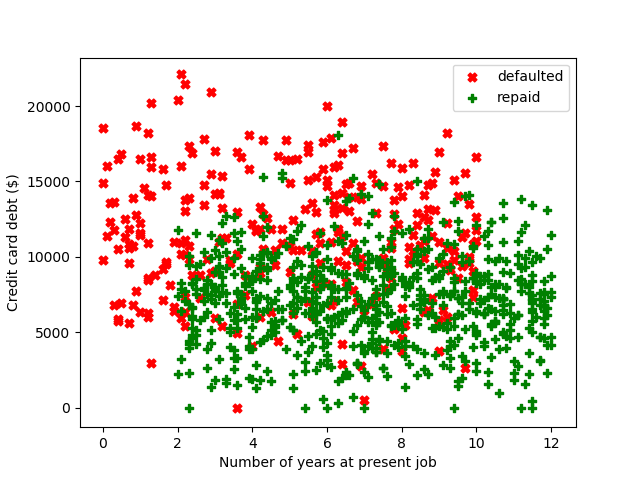
\includegraphics[width=0.85\textwidth]{synthesized_bank.png}
\caption{Synthesized bank data.}
\label{synthesized_bank}
\end{figure}

\section{Coding kNN by hand}

\index{standardization}
\index{normalized (variable)}
\index{Z-score}

To use this as training data, we'll Z-score normalize the features. We also
need to Z-score the \textit{new} data points that come in to be classified,
though, so we'd better remember the mean and standard deviation of each
feature.

\begin{Verbatim}[fontsize=\small,samepage=true,frame=single,framesep=3mm]
def zscores(arr):
    return (arr - arr.mean()) / arr.std()

cc_debt_mean = bank.cc_debt.mean()
cc_debt_std = bank.cc_debt.std()
num_yrs_mean = bank.num_yrs.mean()
num_yrs_std = bank.num_yrs.std()

bank.cc_debt = zscores(bank.cc_debt)
bank.num_yrs = zscores(bank.num_yrs)
\end{Verbatim}
\vspace{-.2in}

\begin{Verbatim}[fontsize=\scriptsize,samepage=true,frame=leftline,framesep=5mm,framerule=1mm]
                  cc_debt   num_yrs default
            0    1.321445  0.152280     yes
            1    0.877662 -0.407452      no
            2    0.150633 -1.000109     yes
            3    2.152262 -1.790319     yes
            4    0.927766  1.238819      no
            ..        ...       ...     ...
            995 -1.450414 -0.670855      no
            996 -0.777325  0.415683      no
            997 -0.172235  0.942490      no
            998  0.385818  0.316907     yes
            999 -0.669958  1.600998      no
\end{Verbatim}

\index{predict@\texttt{predict()}}
\index{dist@\texttt{dist()}}

Now let's write a function called \texttt{predict()} (to match the name we used
in Chapters~\ref{ch:naiveBayes2} and ~\ref{ch:naiveBayes3}) which will make a
loan-default prediction for a new applicant. We'll also write a \texttt{dist()}
(for ``distance'') function to help it do its job.

\index{Euclidean distance}
\index{Pythagorean Theorem}

\begin{Verbatim}[fontsize=\small,samepage=true,frame=single,framesep=3mm]
def dist(x,y):
    return np.sqrt((x[0]-y[0])**2 + (x[1]-y[1])**2)
\end{Verbatim}

We're using Euclidean distance here (Pythagorean Theorem), obviously. Our
\texttt{predict()} will call this \texttt{dist()} function for every point to
determine that point's Euclidean distance from our test point. Then, it will
sort those by distance, pick the top $k$, and choose the majority:

\begin{Verbatim}[fontsize=\small,samepage=true,frame=single,framesep=3mm]
def predict(cc_debt, num_yrs, k):
    bank['dists'] = dist([bank.cc_debt, bank.num_yrs],
        [(cc_debt - cc_debt_mean) / cc_debt_std,
        (num_yrs - num_yrs_mean) / num_yrs_std])
    k_closest_pts = bank.sort_values('dists').iloc[0:k]
    return k_closest_pts.default.value_counts().index[0]
\end{Verbatim}

Can you understand what this function is doing?

First, notice that because of the magic of Pandas broadcasting operations, we
don't even need a loop. The first line of the function calls \texttt{dist()} a
grand total of once, giving it a list of the entire training data's x-values
and y-values as the first argument, and then the new point's x-value and
y-value (both Z-score normalized) as the second argument. Pretty slick!

Then walk through how the majority rule is applied. The variable
``\texttt{k\_closest\_pts},'' after the next line, will be a \texttt{DataFrame}
that looks like so:

\begin{Verbatim}[fontsize=\small,samepage=true,frame=leftline,framesep=5mm,framerule=1mm]
              cc_debt   num_yrs default     dists
        651 -0.058795 -0.720668     yes  0.101662
        254 -0.010493 -0.720668     yes  0.105948
        515  0.057728 -0.854746      no  0.106971
        384  0.076899 -0.821226      no  0.120755
        418 -0.147929 -0.754187     yes  0.123796
        873  0.087356 -0.821226     yes  0.131212
        672 -0.061782 -0.955304      no  0.135271
\end{Verbatim}

\index{value\_counts@\texttt{.value\_counts()} (Pandas)}

(This assumes we passed a value of 7 for the \texttt{k} argument to
\texttt{predict()} and are thus doing 7-NN.) Notice how the rows are ordered in
decreasing distance from our new data point. In the final line of the function,
we take the \texttt{.value\_counts()} of this \texttt{DataFrame}'s
\texttt{default} column. This produces an intermediate value like:

\begin{Verbatim}[fontsize=\small,samepage=true,frame=leftline,framesep=5mm,framerule=1mm]
        yes    4
        no     3
        Name: default, dtype: int64
\end{Verbatim}

and when we take \texttt{.index[0]} of that, we get the label with the
highest value count. In this case, it's ``\texttt{yes},'' so let's not give a
loan to that guy.

\subsection{Evaluating the hand-coded version}

We can measure how well this classifier performs using essentially the same
code we wrote back on p.~\pageref{evaluateNBcode}:

\begin{Verbatim}[fontsize=\small,samepage=true,frame=single,framesep=3mm]
num_correct = 0
for i in range(len(test)):
    row = test.iloc[i]
    p = predict(row['cc_debt'], row['num_yrs'], 3)
    if p == row['default']:
        num_correct += 1
print("We got {}% correct.".format(num_correct/len(test)*100))
\end{Verbatim}
\vspace{-.2in}

\begin{Verbatim}[fontsize=\small,samepage=true,frame=leftline,framesep=5mm,framerule=1mm]
We got 73.667% correct.
\end{Verbatim}

Not that great, but looking again at Figure~\ref{synthesized_bank}
(p.~\pageref{synthesized_bank}) you can see why! There's a huge region in that
space where defaulters and non-defaulters have about the same prominence. For
new points that fall in the midst of that morass, we're only guessing. In a
region like that, no classifier is going to have much of a chance.

%\index{scikit-learn@\texttt{scikit-learn} (package)}
%\section{The \texttt{scikit-learn} library}
%
%
%
%Let's use the scikit-learn library to compare 3-NN with Naive Bayes. First, we
%load the data and split it randomly into training and test sets:
%
%\begin{Verbatim}[fontsize=\footnotesize,samepage=true,frame=single]
%w = pd.read_csv("warriors.csv")
%train = w.sample(frac=.7)
%test = w.drop(train.index)
%\end{Verbatim}
%\normalsize
%
%\vspace{-.05in}
%Next, we one-hot encode the features (all of which are categorical):
%\vspace{-.1in}
%\begin{Verbatim}[fontsize=\footnotesize,samepage=true,frame=single]
%def one_hot_this_puppy(df):
%    lb = LabelBinarizer()
%    lightsaber = lb.fit_transform(df.lightsaber)
%    height = lb.fit_transform(df.height)
%    beard = lb.fit_transform(df.beard)
%    demeanor = lb.fit_transform(df.demeanor)
%    return np.concatenate([lightsaber, height, beard, demeanor], axis=1)
%
%train_features = one_hot_this_puppy(train)
%test_features = one_hot_this_puppy(test)
%\end{Verbatim}
%\normalsize
%
%\vspace{-.05in}
%We'll call scikit-learn's Naive Bayes implementation:
%\vspace{-.15in}
%
%\begin{Verbatim}[fontsize=\footnotesize,samepage=true,frame=single]
%from sklearn.naive_bayes import MultinomialNB
%naive_bayes = MultinomialNB()
%naive_bayes.fit(train_features,train.type.as_matrix())
%nb_predictions = naive_bayes.predict(test_features)
%\end{Verbatim}
%\normalsize
%
%\vspace{-.05in}
%and its KNN implementation:
%\vspace{-.15in}
%
%\begin{Verbatim}[fontsize=\footnotesize,samepage=true,frame=single]
%from sklearn.neighbors import KNeighborsClassifier
%knn = KNeighborsClassifier(n_neighbors=3)
%knn.fit(train_features, train.type.as_matrix())
%knn_predictions = knn.predict(test_features)
%\end{Verbatim}
%\normalsize
%
%\vspace{-.05in}
%Finally, print the results:
%\vspace{-.15in}
%
%\begin{Verbatim}[fontsize=\footnotesize,samepage=true,frame=single]
%>>> print("Naive Bayes got {:.2f}% correct.".format(
%        sum(nb_predictions == test.type)/len(test)*100))
%>>> print("kNN(3) got {:.2f}% correct.".format(
%        sum(knn_predictions == test.type)/len(test)*100))
%    Naive Bayes got 79.00% correct.
%    kNN(3) got 86.33% correct.
%\end{Verbatim}
%\normalsize
%
%Pretty close, but for this data set, 3-NN has the edge.
%
%\subsection{Comparing kNN with Naive Bayes}
%
%\pagebreak
%It's also illustrative to examine \textit{which} points Naive Bayes called
%correctly but 3-NN missed, and vice versa.
%
%\begin{Verbatim}[fontsize=\footnotesize,samepage=true,frame=single]
%nb_right = []
%knn_right = []
%for i in range(len(nb_predictions)):
%    if nb_predictions[i] == test.type.iloc[i] != knn_predictions[i]:
%        nb_right.append(i)
%    if nb_predictions[i] != test.type.iloc[i] == knn_predictions[i]:
%        knn_right.append(i)
%nb_right_examples = test.iloc[nb_right]
%knn_right_examples = test.iloc[knn_right]
%
%>>> print("Naive Bayes got these right:")
%>>> print(nb_right_examples)
%>>> print("\nkNN got these right:")
%>>> print(knn_right_examples)
%\end{Verbatim}
%
%\begin{multicols}{2}
%\begin{Verbatim}[fontsize=\scriptsize,samepage=true,frame=none]
%Naive Bayes got these right:
%    beard  height  demeanor lightsaber  type
%7      no  medium      calm      green  Jedi
%63     no   short  menacing      green  Jedi
%116    no  medium      calm      green  Jedi
%154    no  medium      calm      green  Jedi
%185    no   short  menacing      green  Jedi
%190    no   short  menacing      green  Jedi
%279    no  medium      calm       blue  Jedi
%600    no  medium      calm       blue  Jedi
%827    no   short  menacing      green  Jedi
%842    no   short  menacing      green  Jedi
%909    no   short  menacing      green  Jedi
%\end{Verbatim}
%\columnbreak
%\begin{Verbatim}[fontsize=\scriptsize,samepage=true,frame=none]
%kNN got these right:
%    beard  height  demeanor lightsaber  type
%1      no   short      calm       blue  Sith
%33     no   short      calm       blue  Sith
%55     no   short      calm       blue  Sith
%94     no  medium      calm      green  Sith
%106    no   short      calm       blue  Sith
%254    no   short  menacing      green  Sith
%283    no   short      calm       blue  Sith
%366    no  medium      calm       blue  Sith
%380    no  medium      calm      green  Sith
%385    no  medium      calm       blue  Sith
%431    no   short      calm       blue  Sith
%468    no   short      calm       blue  Sith
%570    no   short      calm       blue  Sith
%581    no   short      calm       blue  Sith
%599    no   short      calm      green  Sith
%686    no  medium      calm      green  Sith
%713    no  medium      calm       blue  Sith
%733    no   short      calm       blue  Sith
%743    no  medium      calm       blue  Sith
%815    no   short  menacing      green  Sith
%870    no   short      calm       blue  Sith
%931    no  medium      calm       blue  Sith
%966    no  medium      calm      green  Sith
%991    no  medium      calm       blue  Sith
%\end{Verbatim}
%\end{multicols}
%\normalsize
%
%Interestingly, all of Naive Bayes's errors were in one direction (incorrect
%\texttt{Jedi} call) and all 3-NN's in the other. Naive Bayes seems to have the
%most trouble with clean-shaven, calm, non-red-lightsabered Sith Lords. It
%tends to call them ``Jedi,'' because two of the features --
%\texttt{demeanor=calm} and \texttt{lightsaber=blue/green} -- are highly
%\texttt{Jedi}-indicative. When factored in with just one
%\texttt{Sith}-indicative feature (\texttt{beard=no}), those two features
%overcome the third and tilt the Naive Bayes scales (incorrectly) towards Jedi.
%3NN is able to pick out these \texttt{Sith} from the \texttt{Jedi} masses.
%
%\subsection{Varying $k$}
%
%One question that arises is: ``what's the
%optimal value of $k$?'' It may or may not surprise you to learn that there's no
%easy answer to this, and that it varies widely by data set and in fact even by
%the training set chosen.
%
%Here's some code to try all (odd) values of $k$ between 1 and 301:
%\begin{Verbatim}[fontsize=\footnotesize,samepage=true,frame=single]
%corrects_train = []
%corrects_test = []
%for k in np.arange(1,301,2):
%    knn = KNeighborsClassifier(n_neighbors=k)
%    knn.fit(train_features, train.type.as_matrix())
%    knn_predictions_train = knn.predict(train_features)
%    knn_predictions_test = knn.predict(test_features)
%    corrects_train.append(sum(knn_predictions_train == train.type)/len(train)*100)
%    corrects_test.append(sum(knn_predictions_test == test.type)/len(test)*100)
%\end{Verbatim}
%\normalsize
%
%The resulting plot is in Figure~\ref{fig:varyingK}. The performance on the
%training data is \textit{usually} better, as expected, although you'll see
%some values of $k$ here in the 80-100 range where paradoxically that's not
%true. More importantly, you'll notice that the line shows no simple pattern.
%Very low numbers are good, and then performance tails off...but then it goes
%back up again when $k$ is around 100 or so. Moreover, \textit{the apparent
%optimal choice of k depends on the training set.}
%
%\begin{figure}
%\centering
%\includegraphics[width=0.9\textwidth]{k_vs_performance.pdf}
%\caption{Correct classification rate as a function of $k$.}
%\label{fig:varyingK}
%\end{figure}
%
%Figure~\ref{fig:varyingTrainingSet} has some more results from the same code,
%with different randomly-chosen training sets. We see some similarities here,
%but by no means perfect uniformity. This is because a kNN classifier is a
%high-variance classifier (especially for low $k$), as described in the next
%section.
%
%\begin{figure}
%\centering
%\includegraphics[width=0.31\textwidth]{k_vs_performance1.pdf}
%\includegraphics[width=0.31\textwidth]{k_vs_performance2.pdf}
%\includegraphics[width=0.31\textwidth]{k_vs_performance3.pdf}
%\caption{Correct classification rate vs.~$k$, for different training sets.}
%\label{fig:varyingTrainingSet}
%\end{figure}
%
%
%\section{The ``Bias-Variance Tradeoff''}
%
%One of the most deep and fundamental principles of machine learning goes by
%the name of \textbf{the bias-variance tradeoff}. It's a version of the ``no
%free lunch'' principle: classifiers that possess one advantage inherently have
%a counteracting disadvantage.
%
%Here are the two key terms:
%
%\begin{itemize}
%\itemsep.1em
%\item \textbf{bias}\footnote{Tip: when thinking about this topic, try to erase the previous definitions you
%have for the word ``\textit{bias}'' that you have running around in your brain.
%They probably don't apply. When I think of ``bias'' I think of a systematic
%propensity to err \textit{in a particular direction}. Like, ``you're biased
%towards thinking people are shorter than they are, because you're tall.'' But
%\textit{bias} here just means ``being `off' in general, in whatever direction,
%and probably not the same direction each time.''}
% -- the degree to which a model is expected to misclassify
%items, even those in its own training set, because it just can't ``bend'' 
%enough to catch all the detail.
%\item \textbf{variance} -- the degree to which a model will differ based on
%the particular training set that is chosen, because it ``bends'' too much to
%try and catch every data point.
%\end{itemize}
%
%The basic theory is as follows. Suppose you have a very simple classifier that
%tries to identify a single, smooth, perfectly straight line separating the
%data points. Maybe our model says ``just use the \texttt{lightsaber} feature
%by itself, and call `\texttt{Jedi}' or `\texttt{Sith}' based on whether the
%test point's lightsaber value is more typical of the \texttt{Jedi} Knights and
%\texttt{Sith} Lords in the data set.
%
%This simple classifier can be said to have \textbf{low variance}. Why? Because
%if, instead of those particular 714 training points chosen from the
%population, I had sampled a different 714 training points, \textit{the
%classification decisions I would make on new data would be about the same.} To
%see why this is the case, consider how different the training sets would have
%to me in order for me to make any \textit{different} decisions. Let's say my
%original 714 training points had:
%
%\begin{center}
%\begin{Verbatim}[fontsize=\small,samepage=true,frame=none]
%        Jedi    Sith
%red       17      85
%blue     283      28
%green    299       2
%\end{Verbatim}
%\end{center}
%
%for their lightsaber colors. Clearly, my very simply classifier is going to
%predict \texttt{Sith} for any \texttt{red}-lightsaber wielder and
%\texttt{Jedi} for anyone else. Now if I had collected a different training
%set, the numbers above would be different, but they would have to be a
%\textit{lot} different to change any of my future predictions. I'd have to
%have an additional 68 \texttt{red} \texttt{Jedi}, for instance, or 255
%additional \texttt{blue} \texttt{Sith}, or a whopping 297 additional
%\texttt{green} \texttt{Sith}, without any increase in the other class. Not
%likely.
%
%That's the bright side. On the dark side, by classifying points in this way,
%this simple model is going to get a lot of data points wrong: $17+28+2=47$
%points incorrect \textit{in its own training set}, in fact. This mean it's a
%pretty \textbf{high bias} classifier.
%
%It's a tradeoff. In exchange for being virtually immune to the idiosyncrasies
%in the training sample, we've sacrificed some precision.
%
%The other extreme can be seen by visualizing a 1-NN classifier. Now, for a
%future data point, we're going to find the single nearest neighbor to it in
%our training set, and call \texttt{Jedi} or \texttt{Sith} accordingly. This is
%very \textbf{low bias} -- we're guaranteed to get every training point
%correct, in fact!\footnote{Unless there are data points with identical feature
%values but different labels, in which case whatcha gonna do.} But it is also
%very \textbf{high variance}: a different training set will result in many,
%many different classifications. Our classifier has essentially memorized a
%zillion individual examples, and will regurgitate all that intricate detail on
%command. But had we gotten a different random sample, the ``single nearest
%neighbor'' to a test point would have been totally different, and might result
%in a different classification.
%     
%There are formulas you can use to work out quantitatively what the estimated
%bias and variance are for a classifier. But I think this dichotomy is more
%important from a conceptual perspective. The main lesson is: the more your
%classifier ``bends'' (\textit{i.e.}, has a very wiggly and unpredictable
%boundary between its ranges of predicted classes) the more precise it
%potentially is in selectively labeling data points. However, this also means
%that a lot of its decisions are going to hinge on the particular data sample
%it was trained on, which means it will probably be picking up noise in
%addition to signal.
%
%
%\section{The ``Curse of Dimensionality''}
%\label{sec:curse}
%
%Another key ML principle goes by the humorous name \textbf{the curse of
%dimensionality}. It goes something like this. Suppose that in addition to
%\texttt{height}, \texttt{demeanor}, \texttt{lightsaber}, and \texttt{beard},
%we also have at our disposal many other features about Jedi \& Sith: their
%ages, salaries, home planets, personality profiles, number of traffic tickets,
%\textit{etc.} This is good news, right? It gives us more and more data to sift
%through statistically and discover correlations, right? What's not to like?
%
%Yes, this is potentially good news, but with a catch. It turns out that as we
%increase the number of features more and more (or, put another way, as we
%increase the ``dimensionality'' of the problem from our original four
%dimensions to 5, 6, 7, ..., and up into the hundreds) we have a data sparsity
%problem. In terms of kNN classifiers, you can think of it this way:
%effectively, \textit{all} the points effectively become far apart. We want to
%find the 3 (or 15, or 77) ``nearest neighbors,'' but when we have so many
%features (many of which will turn out to be irrelevant for the problem), we
%find that \textit{any} two data points will differ on a large number of them.
%Essentially, our noise swamps our signal.
%
%Another aspect of the problem concerns the amount of training data that we
%need. When we have tons of features, we need an enormous number of training
%samples in order to guarantee that we have several samples with each
%combination of values (or their ranges). In our original problem, we didn't
%need to much data to ensure that we'd have at least a few \texttt{tall},
%\texttt{green}-lightsabered, \texttt{menacing} individuals with \texttt{no}
%beard. But how many training points will we need before we have several
%\texttt{tall}, \texttt{green}-lightsabered, \texttt{menacing}, 38-year-old,
%extroverted, abstract-thinking individuals from Tatooine with 4 traffic
%tickets and \texttt{no} beard who earn 6,000 Galactic credits annually?
%Answer: a lot. And if we don't have that many, a kNN classifier trained on all
%those features is going to suffer trying to find ``people like this one'' in
%order to make a prediction.
%
%The moral to the story is that we will often need to trim our set of features,
%sometimes aggressively, if we have too many. It feels wasteful -- all this
%great data on all these people, and we're throwing it away! -- but it's the
%right thing to do. This process is called \textbf{feature selection}, and
%we'll cover it more fully in a future lesson.
%
%\vspace{.1in}
%In the meantime, here are three useful principles for avoiding the curse:
%
%\begin{itemize}
%\itemsep.1em
%\item By far the most important thing to recognize is that if you have
%additional features that are \textit{truly} (and pretty strongly) correlated
%with the target, it's okay to include them. Adding more stuff that actually
%contains useful information for prediction isn't generally a problem. The
%problem is when you add features that are largely \textit{noise}, since
%they will overwhelm the truly significant features if there are too many of
%them.
%\item A common rule of thumb is to make sure you have at least \textit{five}
%training points for each combination of feature values. (In our Jedi example,
%with three \texttt{height}s and three \texttt{lightsaber} values and two
%values for the other features, this would imply a training set of at least $(3
%\times 3 \times 2 \times 2) \times 5 = 180$ training points.)
%\item When the size of the training set becomes too low, use
%\textit{parametric} methods (like Naive Bayes or linear regression) rather
%than instance-based methods (like kNN) because they suffer less from the
%curse.
%\end{itemize}
%
%
